\section*{Описание экспериментальной установки}

Определение фокусных расстояний собирающих линз методом Аббе:

\begin{figure}[H]
	\centering
	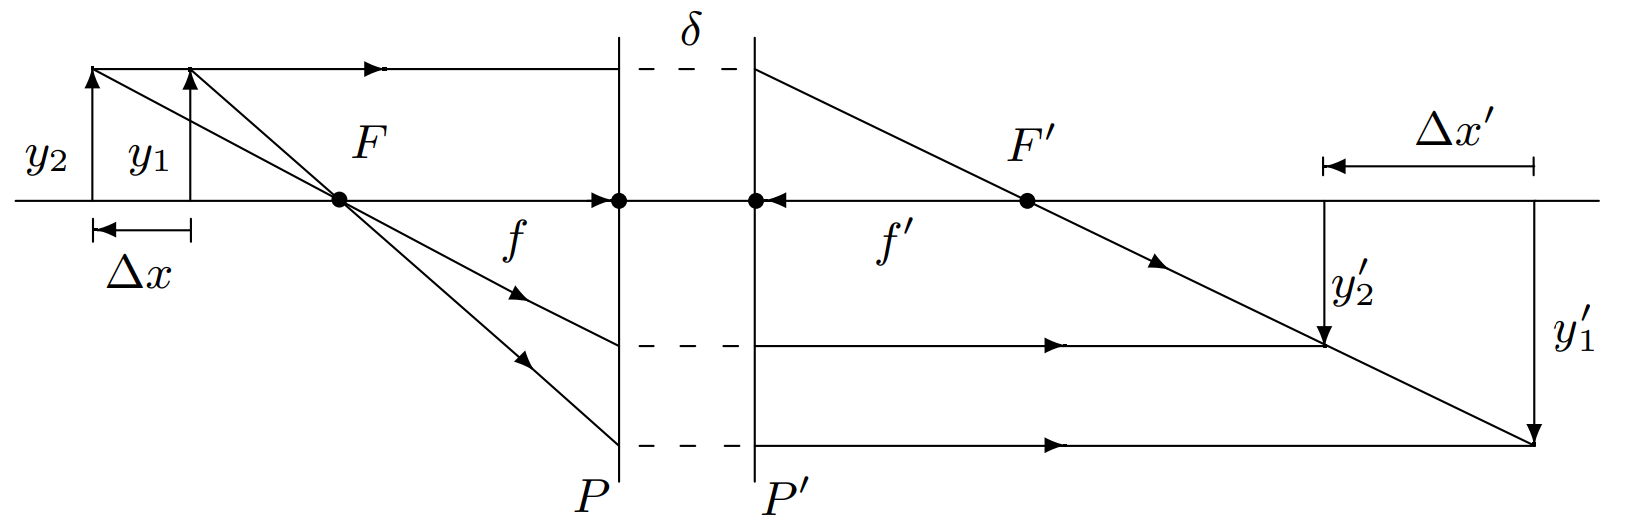
\includegraphics[width=0.5\textwidth]{../Изображения/Аббе.png}
	\caption{Схема экспериментальной установки}
\end{figure}

Рассматривается несколько различных положений источника на оптической оси статичной линзы. Из геометрической оптики следует связь между его сдвигом и изменением продольного увеличения изображения: \\
Передний фокус $f = \frac{\Delta x}{\Delta (y/y')}$ \\
Задний фокус $f = \frac{\Delta x'}{\Delta (y'/y)}$ \\

Определение фокусных расстояний собирающих линз методом Бесселя:

\begin{figure}[H]
	\centering
	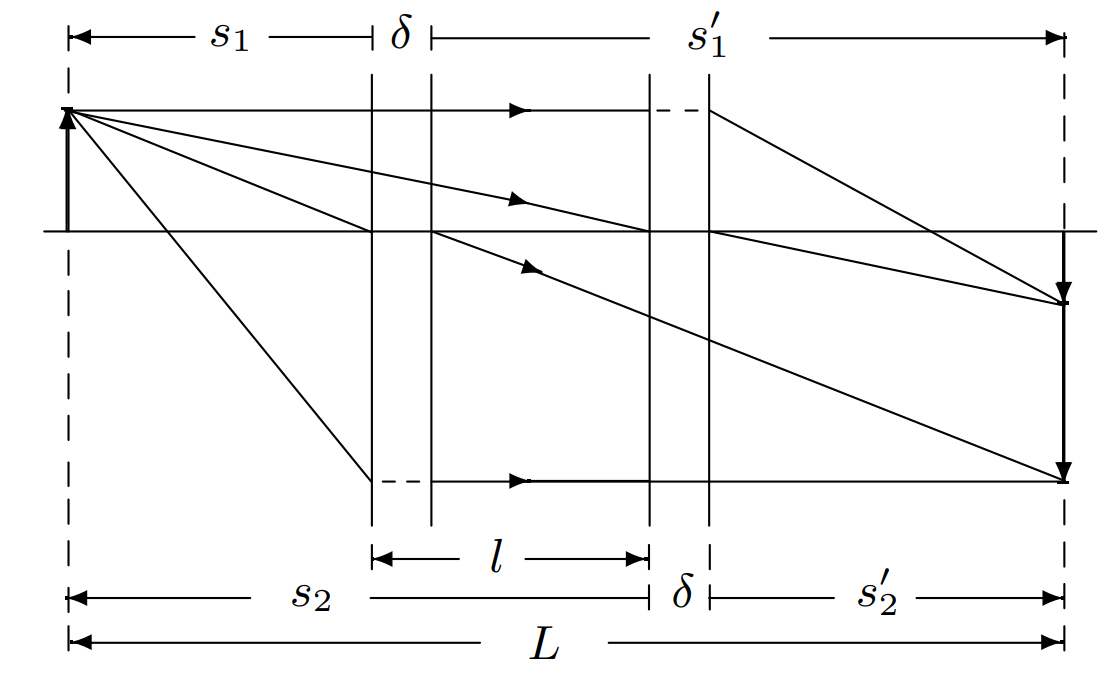
\includegraphics[width=0.5\textwidth]{../Изображения/Бессель.png}
	\caption{Схема экспериментальной установки}
\end{figure}

В методе Бесселя при постоянном расстоянии от источника до экрана находятся два положения линзы, при которых получается чёткое изображение. Фокусное расстояния определяется по формуле:\\
$$f = \frac{(L - \delta)^2 - l^2}{4(L - \delta)}$$
В приближении $\delta << L$, где $\delta$ -- толщина линзы фокусное расстояние вычисляется по формуле: \\
$$f = \frac{L^{2} - l^{2}}{4L}$$
При этом возникает следующая погрешность приближения:
$$\varepsilon_f = \frac{L^2 + l^2}{L^2 - l^2} \frac{|\delta|}{L}$$

Ислледование системы из двух собирающих линз:

\begin{figure}[H]
	\centering
	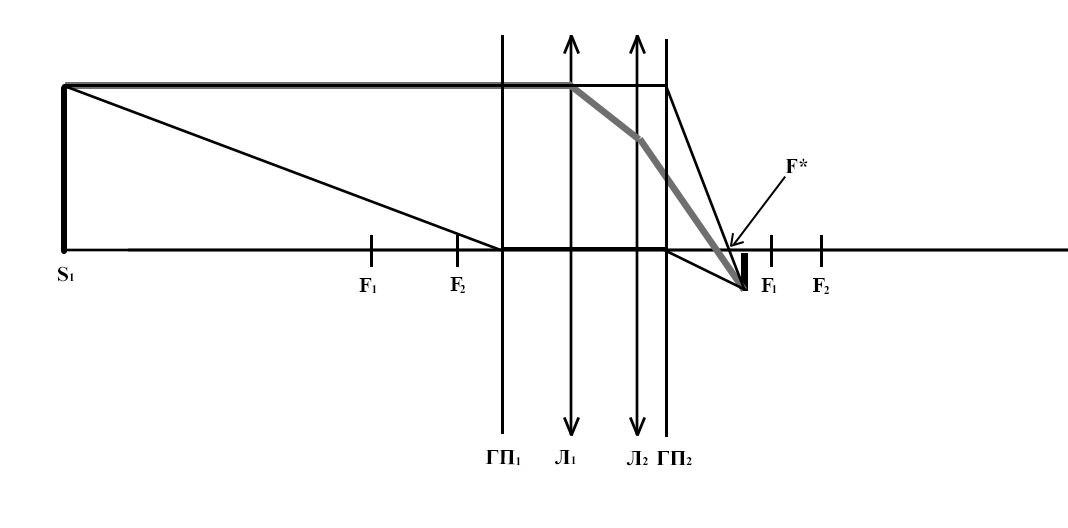
\includegraphics[width=0.5\textwidth]{../Изображения/Система собирающих.png}
	\caption{Схема экспериментальной установки}
\end{figure}


Определение фокусного расстояния рассеивающей линзы в сложной системе:

\begin{figure}[H]
	\centering
	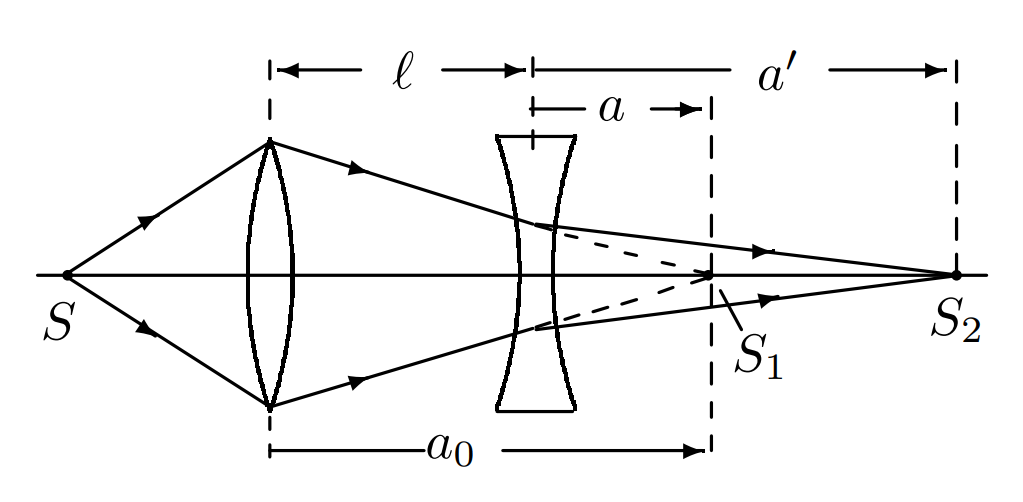
\includegraphics[width=0.5\textwidth]{../Изображения/Фокус рассеивающей.png}
	\caption{Схема экспериментальной установки}
\end{figure}

Фокусное расстояние рассеивающей линзы определяется двумя способами:\\
$\mathbf{Способ 1:}$ С помощью собирающей линзы получают действительное изображение источника. Затем между линзой и изображением ставится рассеивающая линза, таким образом для неё изображение становится мнимым источником и изображение от системы остается действительным. Последнее находится с помощью экрана и из расстояний в системе определяется фокусное расстояние.\\
$\mathbf{Способ 2:}$ Система выглядит так же, только рассеивающая линза располагается так, что изображение от собирающей попадает в её фокальную плоскость. В такой конфигурации лучи после неё уходят параллельным пучком, и чтобы найти такое положение, в конец скамьи ставится зрительная труба, настроенная на бесконечность. Тогда фокусное расстояние линзы есть ни что иное, как расстояние между экраном, на котором фокусируется изображение от одной собирающей линзы и полученным положением рассеивающей.\\
